%% ==============================
\chapter{Methoden der Dimensionsreduktion}
\label{ch:MethodenDerDimRed}
%% ==============================

Nachdem wir nun die Motivation und Idee hinter der Dimensionsreduktion in \chapref{ch:Enleitung} und die mathematische Formulierung
in \chapref{ch:Dimensionsreduktion} allgemein angeschaut haben,
werden nun einige Methoden zur Dimensionsreduktion vorgestellt.

In jüngster Zeit haben vor allem verschiedenste Varianten von neuronale Netzen einen hohen Grad an Aufmerksamkeit durch bahnbrechende Errungenschaften in Gebieten der Spracherkennung oder \textit{Computer Vision} erlangt. Fraglich ist, ob diese neuen Algorithmen auch auf dem Bereich der Dimensionsreduktion einen entscheidenden Fortschritt gemacht haben. Deshalb unterteilen wir die Algorithmen in \textit{traditionelle}
und \textit{moderne} Methoden, um diese später in \chapref{ch:Vergleich} gegenüberstellen zu können. Mit traditionellen Methoden
sind statistische Methoden wie die Hauptkomponentenanalyse (\subsecref{ch:MethodenDerDimRed:traditionell:PCA}) oder andere etablierte
Methoden der Dimensionsreduktion gemeint, wohingegen moderne Methoden auf neuere Entwicklungen wie neuronale Netze und die Varianten davon abzielt. Allerdings ist hier aus jeder Kategorie nur eine kleine repräsentative Auswahl getroffen worden. Weitere wichtige Algorithmen, die hier nicht vorgestellt werden können sind beispielsweise \dots \todo{Nachweise für Algorithmen + aufzählen}.

\section{Traditionelle Methoden}
\label{ch:MethodenDerDimRed:traditionell}

Zuerst widmen wir uns den traditionellen Methoden der Dimensionsreduktion.
Dazu gehören die \newterm{Hauptkomponentenanalyse} (engl. \textit{principal components analysis} (PCA)) in \subsecref{ch:MethodenDerDimRed:traditionell:PCA},
die nicht-lineare Erweiterung der
Hauptkomponentenanalyse (\subsecref{ch:MethodenDerDimRed:traditionell:kPCA})
und die für die Visualisierung sehr verbreitete Methode \newterm{t-distributed stochastic neighborhood embedding} (t-SNE) in \subsecref{ch:MethodenDerDimRed:traditionell:t-SNE}.

%% ==============================
\subsection{Principal Component Analysis}
\label{ch:MethodenDerDimRed:traditionell:PCA}
\nomenclature[Z]{PCA}{Principal Component Analysis}

Principal Component Analysis ist \textit{die} Methode der Dimensionsreduktion und wurde erstmals von \textcite{Pearson.1901} und Hotelling 1933\addref entwickelt. Trotz des mittlerweile relativ hohen Alters ist die Hauptkomponentenanalyse immer noch aufgrund der simplen Anwendbarkeit oft die erste Wahl einer Dimensionsreduktionsmethode. Im Folgenden möchte ich kurz auf die zentrale Idee und Motivation (\ref{ch:MethodenDerDimRed:traditionell:PCA:Grundidee}) der Hauptkomponentenanalyse, sowie die mathematische Herleitung der sogenannten \newterm{Hauptkomponenten} (\ref{ch:MethodenDerDimRed:traditionell:PCA:Herleitung}) eingehen.


\subsubsection{Grundidee}
\label{ch:MethodenDerDimRed:traditionell:PCA:Grundidee}
Die zentrale Idee der Hauptkomponentenanalyse ist die Transformation des Koordinatensystems in einer möglichst \textit{verlustfreien} Art und Weise. Verlustfrei bedeutet im Kontext der Hauptkomponentenanalyse, dass möglichst viel Variation in den Daten erhalten bleiben soll \parencite[vgl.][1]{Jolliffe.2002}. Möchte man dann die Dimension von $D$ auf die intrinsische Dimension $d$ reduzieren wählt man einfach die \textit{ersten} $d$ Hauptkomponenten. Was diese Hauptkomponenten sind, werden wir im nächsten Abschnitt genauer sehen.

\subsubsection{Herleitung der Hauptkomponenten}
\label{ch:MethodenDerDimRed:traditionell:PCA:Herleitung}
Wir haben also als Ausgangsbasis einen $D$-dimensionalen Zufallsvektor $\rvect{x} = \tr{(\rv{x}_1, \ldots, \rv{x}_D)}$ und unser Ziel ist es, eine $d$-dimensionale Repräsentation $\rvect{y}$ zu erhalten. Dabei drücken wir nun $\rvect{y}$ als eine Linearkombination des ursprünglichen hochdimensionalen Vektors $\rvect{x}$ wie folgt aus:
\begin{equation}
	\rvect{y} = \sc{a}_1 \rv{x}_1 + \cdots + \sc{a}_D \rv{x}_D
\end{equation}

%% ==============================
\subsection{Kernel Principal Component Analysis}
\label{ch:MethodenDerDimRed:traditionell:kPCA}
\nomenclature[Z]{kPCA}{Kernel Principal Component Analysis}

%% ==============================
\subsection{t-distributed Stochastic Neighborhood Embedding}
\label{ch:MethodenDerDimRed:traditionell:t-SNE}
\nomenclature[Z]{t-SNE}{t-distributed Stochastic Neighborhood Embedding}

\newpage

%% ==============================
%% ==============================
\section{Moderne Methoden}
\label{ch:MethodenDerDimRed:modern}
%% ==============================
Hier werden Moderne Methoden vorgestellt.

\subsection{Autoencoder}
\label{ch:MethodenDerDimRed:modern:AE}
\nomenclature[Z]{AE}{Autoencoder}

\begin{figure}[h]
	\label{fig:5-layer-Autoencoder}
	\begin{center}
		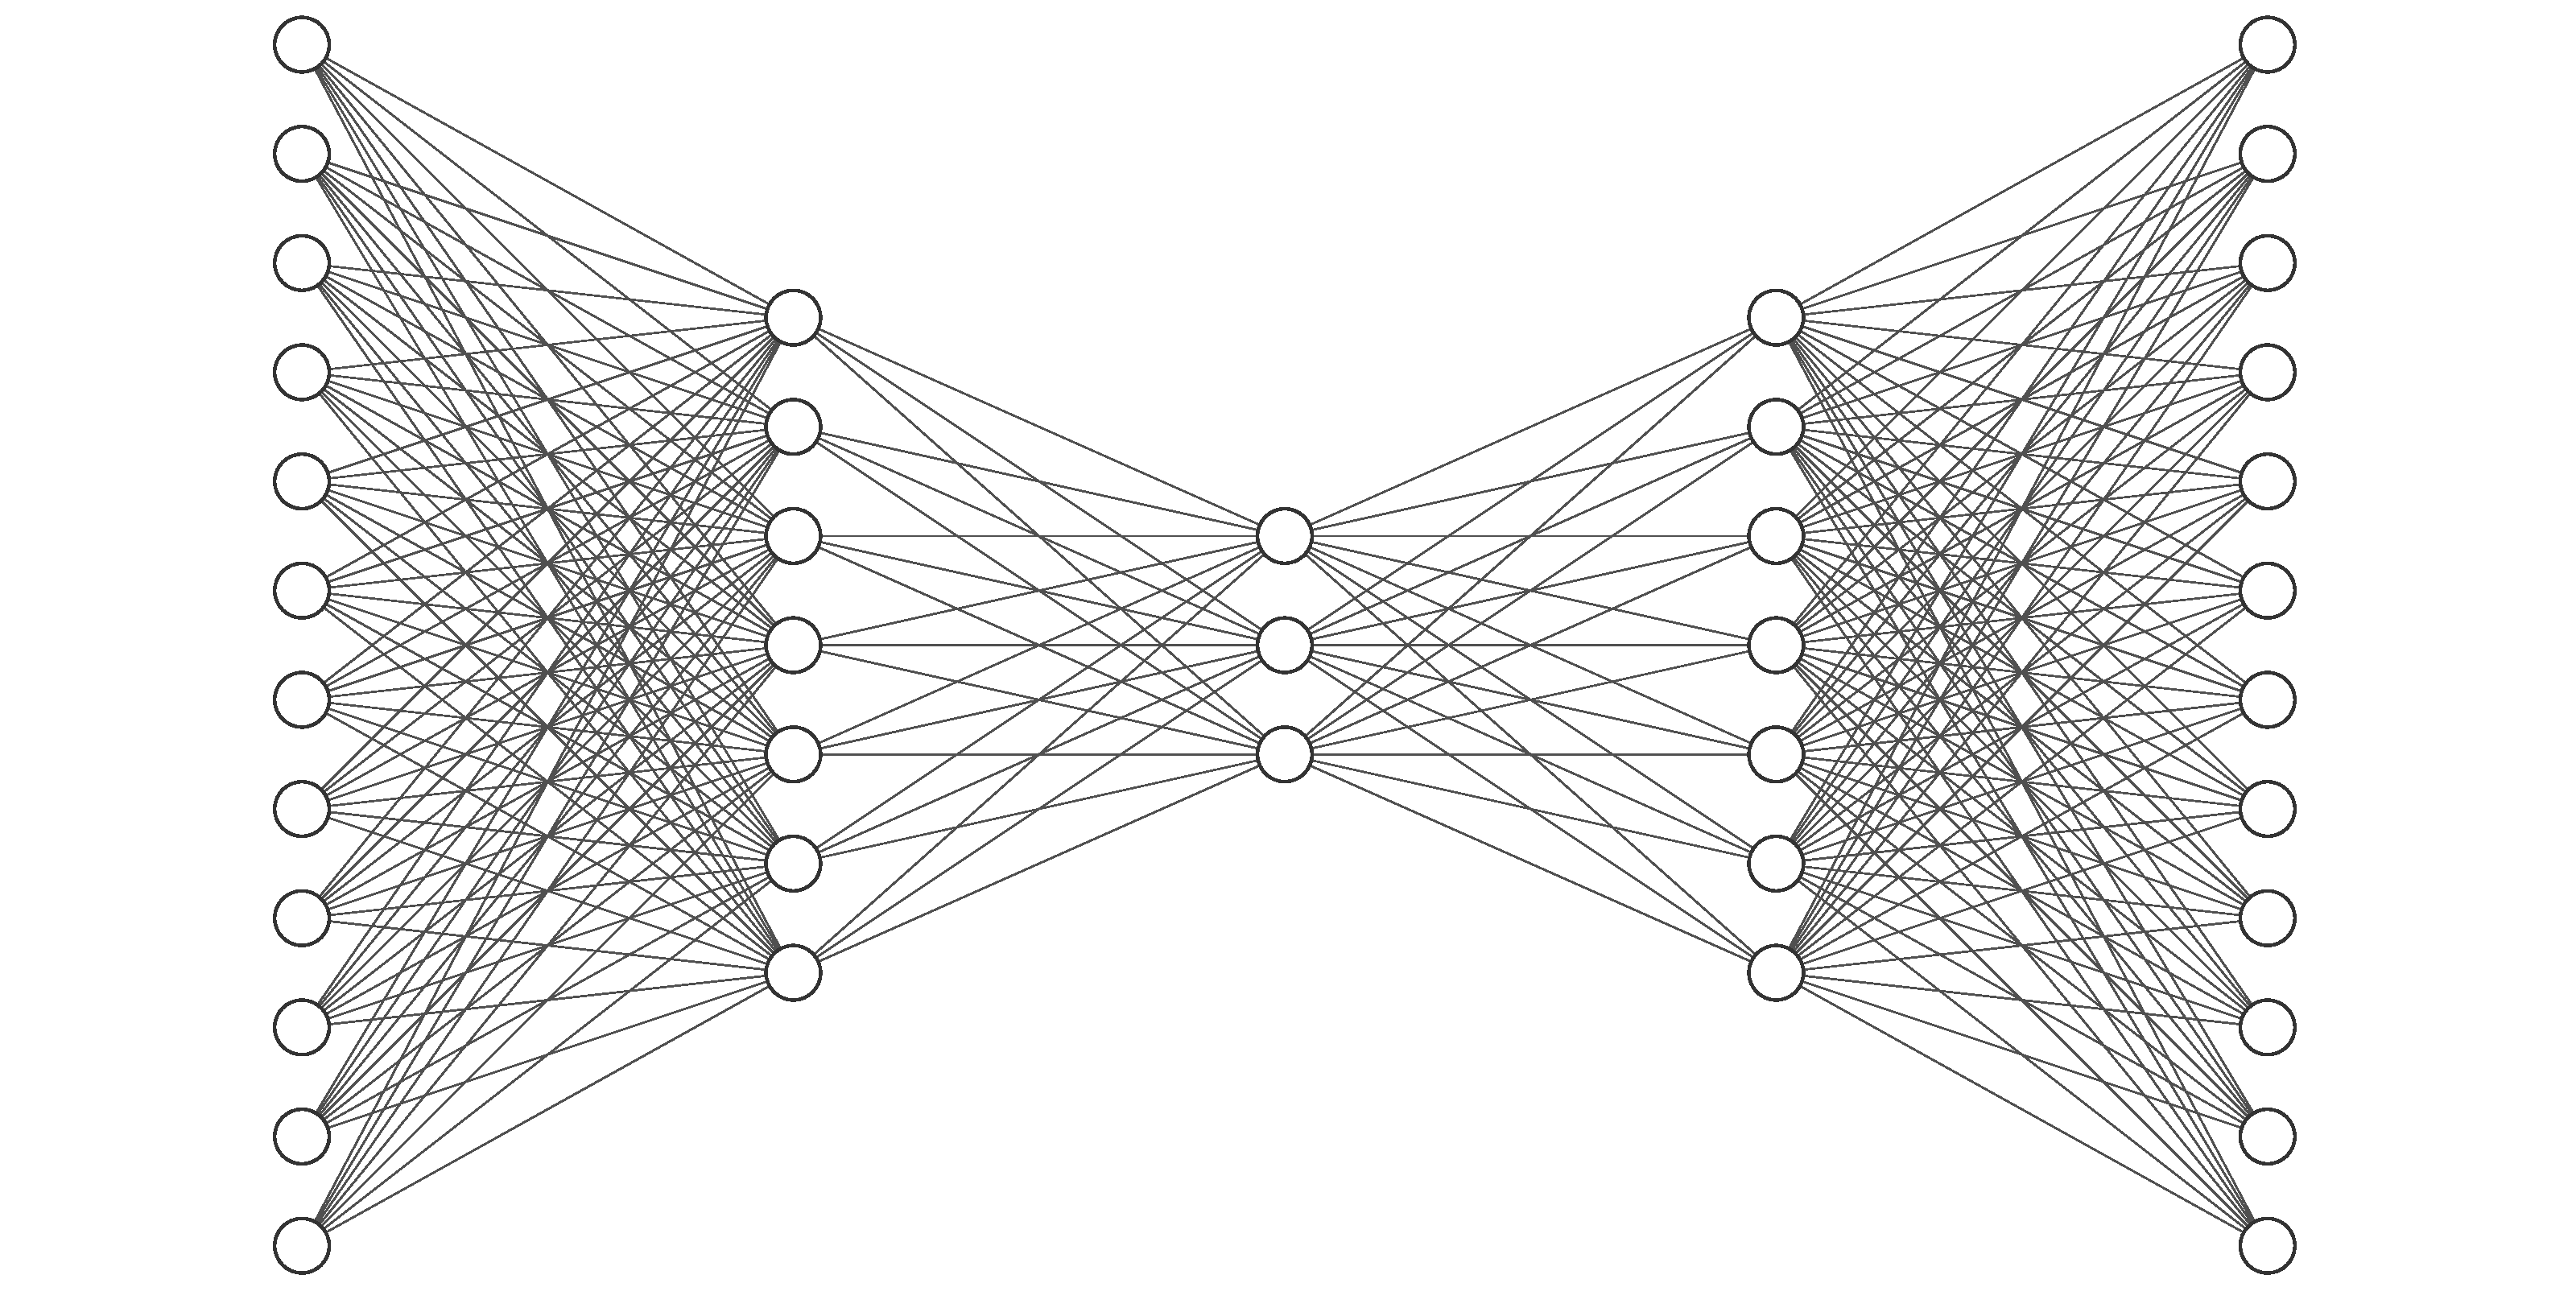
\includegraphics[width=\textwidth]{5_layer_AE.pdf}
		\caption[Schematische Abbildung der Architektur eines Autoencoders]{Gezeigt ist eine schematische Abbildung der Architektur eines Autoencoders. Dieser Autoencoder besitzt fünf Schichten, wobei das \textit{Bottleneck} dreidimensional und die \textit{Input}-Dimension zwölf ist. Das bedeutet, dass ein 12-dimensionaler Inputvektor in der Mitte des Autoencoders durch einen dreidimensionalen Vektor kodiert und anschließend wieder dekodiert werden muss, um zu einer möglichst verlustfreien Rekonstruktion zu gelangen.}
	\end{center}
\end{figure}

\subsection{Variational Autoencoder}
\label{ch:MethodenDerDimRed:modern:VAE}
\nomenclature[Z]{VAE}{Variational Autoencoder}

\subsection{Self-Organizing Maps}
\label{ch:MethodenDerDimRed:modern:SOM}
\nomenclature[Z]{SOM}{Self-Organizing Map}
